% (c) 2016 Elisabetta Campana
% (c) 2016 Daniele Zambelli daniele.zambelli@gmail.com

\section{Esercizi}

\subsection{Esercizi dei singoli paragrafi}

\subsubsection*{\numnameref{sec:irvalass_supsec}}

% \begin{esercizio}
% \label{ese:D.19}
% testo esercizio
% \end{esercizio}

\begin{esercizio}\label{ese:03.1}
Risolvi le seguenti equazioni:
\begin{enumeratea}
\item $9\,{x}^{8}-108\,{x}^{4}+360=0$ 
\hfill [$\not\exists x \in \mathbb{R}$]
\item $9\,{x}^{8}-72\,{x}^{4}+144=324$ 
\hfill [$(x=-\sqrt [4]{10})\vee (x=\sqrt [4]{10})$]
\item $-9=-64\, \left( 5\,x-2 \right) ^{6}$ 
\hfill [$(x={\dfrac{\sqrt [3]{3}}{10}}+{\dfrac{2}{5}})\vee (x=-{\dfrac
{\sqrt 
[3]{3}}{10}}+{\dfrac{2}{5}})$]
\item $729\, \left( x+1 \right) ^{6}+2=0$ 
\hfill [$\not\exists x \in \mathbb{R}$]
\item $243\,{x}^{5}=-9$ 
\hfill [$x=-{\dfrac{{3}^{{\frac{2}{5}}}}{3}}$]
% \item $0= \left( 9\,x-7 \right) ^{5}-9$ 
% \hfill [$x={\dfrac{{3}^{{\frac{2}{5}}}}{9}}+{\dfrac{7}{9}}$]
\item $6\,{x}^{10}-96\,{x}^{5}+234=0$ 
\hfill [$(x=\sqrt [5]{3})\vee (x=\sqrt [5]{13})$]
\item $-8\,{x}^{8}-392=112\,{x}^{4}-72$ 
\hfill [$\not\exists x \in \mathbb{R}$]
\item $78=-3\,{x}^{10}+6\,{x}^{5}$ 
\hfill [$\not\exists x \in \mathbb{R}$]
\item $-70\,{x}^{4}+175=-7\,{x}^{8}-448$ 
\hfill [$\not\exists x \in \mathbb{R}$]
% \item $- \left( 5\,x-9 \right) ^{7}=-9$ 
% \hfill [$x={\dfrac{{3}^{{\frac{2}{7}}}}{5}}+{\dfrac{9}{5}}$]
% \item $-7\,{x}^{2}=-x \left( {x}^{3}-10\,{x}^{2}+70 \right) $ 
% \hfill [$(x=0)\vee (x=10)\vee (x=\sqrt {7})\vee (x=-\sqrt {7})$]
\item $-8\,{x}^{10}-32\,{x}^{5}=160$ 
\hfill [$\not\exists x \in \mathbb{R}$]
\item $-7\,{x}^{10}+140\,{x}^{5}-700=0$ 
\hfill [$x=\sqrt [5]{10}$]
\item $-56\,{x}^{4}-679=7\,{x}^{8}$ 
\hfill [$\not\exists x \in \mathbb{R}$]
\item ${x}^{4}-13\,{x}^{3}-13\,x+40=-41\,{x}^{2}$ 
\hfill [$(x=5)\vee (x=8)$]
\item $1024\,{x}^{5}-8=0$ 
\hfill [$x={\dfrac{{2}^{{\frac{3}{5}}}}{4}}$]
% \item $16\,{x}^{5}+36={x}^{10}+64$ 
% \hfill [$(x=\sqrt [5]{2})\vee (x=\sqrt [5]{14})$]
\item $x \left( {x}^{3}+6 \right) =-6\,{x}^{3}-9\,{x}^{2}-8$ 
\hfill [$(x=-4)\vee (x=-2)$]
\item ${x}^{4}-72\,x+120=2\,{x}^{2} \left( 6\,x-13 \right) $ 
\hfill [$(x=2)\vee (x=10)$]
\item $0=-6\,{x}^{8}-24\,{x}^{4}+462$ 
\hfill [$(x=-\sqrt [4]{7})\vee (x=\sqrt [4]{7})$]
\item $ \left( x+9 \right) ^{6}-4=0$ 
\hfill [$(x=\sqrt [3]{2}-9)\vee (x=-\sqrt [3]{2}-9)$]
\item $128\,{x}^{3}+800=-8\,{x}^{6}$ 
\hfill [$\not\exists x \in \mathbb{R}$]
% \item $5\,{x}^{8}-40=0$ 
% \hfill [$(x=-{2}^{{\frac{3}{8}}})\vee (x={2}^{{\frac{3}{8}}})$]
% \item $0=2\,{x}^{10}-8\,{x}^{5}+8$ 
% \hfill [$x=\sqrt [5]{2}$]
% \item $108\,{x}^{4}=9\,{x}^{8}+324$ 
% \hfill [$(x=-\sqrt [4]{6})\vee (x=\sqrt [4]{6})$]
\end{enumeratea}
\end{esercizio}

\begin{esercizio}\label{ese:03.1}
Risolvi le seguenti equazioni:
\begin{enumeratea}
\item $-{\dfrac{ \left( x+15 \right) ^{5}}{9^5}}= \left( 4\,x-5 \right) 
^{5}$ 
\hfill [$x={\dfrac{30}{37}}$]
\item ${\dfrac{{x}^{10}}{5}}=-{\dfrac{3\,{x}^{5}}{4}}-{\dfrac{65}{64}}$ 
\hfill [$\not\exists x \in \mathbb{R}$]
\item ${x}^{3}-{\dfrac{5}{28}}={\dfrac{7\,{x}^{6}}{5}}$ 
\hfill [$x={\dfrac{\sqrt [3]{980}}{14}}$]
% \item ${\dfrac{7\,{x}^{8}}{10}}=-{\dfrac{{x}^{4}}{9}}+{\dfrac
% {1615}{1134}}$ 
% \hfill [$(x=-{\dfrac{{7}^{{\frac{3}{4}}}\sqrt {3}\sqrt 
% [4]{85}}{21}})\vee 
% (x={\dfrac{{7}^{{\frac{3}{4}}}\sqrt {3}\sqrt [4]{85}}{21}})$]
\item ${\dfrac{ \left( 9\,x-32 \right) ^{4}}{12^4}}=-2$ 
\hfill [$\not\exists x \in \mathbb{R}$]
% \item ${x}^{4}+{\dfrac{62\,{x}^{2}}{7}}-{\dfrac{88\,x}{7}}-{\dfrac
% {80}{7}}=-11\,{x}^{3}$ 
% \hfill [$(x=-10)\vee (x=-1)\vee (x={\dfrac{2 \sqrt {14}}{7}})\vee 
% (x=-{\dfrac{2 \sqrt {14}}{7}})$]
% \item ${\dfrac{x \left( 4\,{x}^{3}+31\,x+63 \right) 
% }{4}}=7\,{x}^{3}+{\dfrac{45}{2}}$ 
% \hfill [$(x=5)\vee (x=-{\dfrac{3}{2}})\vee (x=2)\vee (x={\dfrac{3}{2}})$]
\item $-{\dfrac{4}{5}}={\dfrac{9\,{x}^{6}}{5}}$ 
\hfill [$\not\exists x \in \mathbb{R}$]
\item $0={\dfrac{{x}^{10}}{2}}-{\dfrac{{x}^{5}}{2}}+{\dfrac{401}{8}}$ 
\hfill [$\not\exists x \in \mathbb{R}$]
\item $0={\dfrac{ \left( 35\,x-18 \right) ^{5}}{24}}$ 
\hfill [$x={\dfrac{18}{35}}$]
\item ${x}^{4}-{\dfrac{601\,{x}^{2}}{10}}-{\dfrac
{2\,x}{5}}+6=-4\,{x}^{3}$ 
\hfill [$(x=-10)\vee (x=6)\vee (x={\dfrac{\sqrt {10}}{10}})\vee 
(x=-{\dfrac
{\sqrt {10}}{10}})$]
\item $-90=-{\dfrac{x \left( 3\,{x}^{3}+45\,{x}^{2}+157\,x-75 \right) 
}{3}}$ 
\hfill [$(x=-9)\vee (x=-6)\vee (x={\dfrac{\sqrt {15}}{3}})\vee (x=-{\dfrac
{\sqrt 
{15}}{3}})$]
\item $0={\dfrac{ \left( 35\,x-16 \right) ^{7}}{40^7}}-{\dfrac{1}{2}}$ 
\hfill [$x={\dfrac{4 {2}^{6/7}}{7}}+{\dfrac{16}{35}}$]
\item ${\dfrac{2}{9}}=-{\dfrac{ \left( 9\,x-56 \right) ^{8}}{5}}$ 
\hfill [$\not\exists x \in \mathbb{R}$]
\item $-{\dfrac{512\, \left( 25\,x-14 \right) ^{9}}{35^9}}+4=0$ 
\hfill [$x={\dfrac{7 {2}^{2/9}}{10}}+{\dfrac{14}{25}}$]
\item ${\dfrac{5\,{x}^{8}}{7}}+{\dfrac{3\,{x}^{4}}{2}}=-{\dfrac
{91}{80}}$ 
\hfill [$\not\exists x \in \mathbb{R}$]
\item ${\dfrac{ \left( 81\,x+80 \right) ^{7}}{72^7}}=- \left( x-1 
\right) ^{7}$ 
\hfill [$x=-{\dfrac{8}{153}}$]
\item $0=-{\dfrac{ \left( 9\,x-5 \right) ^{4}}{6561}}$ 
\hfill [$x={\dfrac{5}{9}}$]
\item ${\dfrac{ \left( 9\,x-10 \right) ^{3}}{15^3}}=- \left( 9\,x+7 
\right) 
^{3}$ 
\hfill [$x=-{\dfrac{95}{144}}$]
\item ${\dfrac{3\,{x}^{3}}{7}}={\dfrac{4\,{x}^{6}}{5}}+{\dfrac
{24545}{28^2}}$ 
\hfill [$\not\exists x \in \mathbb{R}$]
\item ${\dfrac{1}{486}}=-6\,{x}^{10}-{\dfrac{2\,{x}^{5}}{9}}$ 
\hfill [$x=-{\dfrac{{12}^{{\frac{2}{5}}}}{6}}$]
% \item $-{\dfrac{ \left( 3\,x-2 \right)  \left( 4\,{x}^{2}-x-2 \right) 
% }{3}}=-{x}^{4}$ 
% \hfill [$(x={\dfrac{\sqrt {3}}{3}})\vee (x=-{\dfrac{\sqrt {3}}{3}})\vee 
% (x=2)$]
\item ${\dfrac{4\,{x}^{3}}{3}}-{\dfrac{16}{81}}={\dfrac
{9\,{x}^{6}}{4}}-{\dfrac{100}{9}}$ 
\hfill [$(x={\dfrac{\sqrt [3]{68}}{3}})\vee (x=-{\dfrac{\sqrt 
[3]{52}}{3}})$]
\end{enumeratea}
\end{esercizio}

\begin{esercizio}\label{ese:03.1}
Risolvi le seguenti disequazioni:
\begin{enumeratea}
% \item $5^9\, \left( x-1 \right) ^{9}+512\, \left( 2\,x-1 \right) ^{9}>0$ 
% \hfill [${\dfrac{7}{9}}<x$]
% \item $-168\geq 3\,{x}^{6}+54\,{x}^{3}$ 
% \hfill [$x\leq -{2}^{{\frac{2}{3}}} \wedge -\sqrt [3]{14}\leq x$]
\item $4\,{x}^{6}-48\,{x}^{3}+144\leq 324$ 
\hfill [$x\leq \sqrt [3]{15} \wedge -\sqrt [3]{3}\leq x$]
\item $-8\, \left( 3\,x-1 \right) ^{3}> \left( 7\,x+4 \right) ^{3}$ 
\hfill [$x<-{\dfrac{2}{13}}$]
\item $0\geq  \left( 10\,x-7 \right) ^{5}-1$ 
\hfill [$x\leq {\dfrac{4}{5}}$]
\item $-{x}^{3}\geq -1$ 
\hfill [$x\leq 1$]
\item $-5\,{x}^{9}+40\geq 0$ 
\hfill [$x\leq \sqrt [3]{2}$]
\item $9\,{x}^{10}+900\geq 180\,{x}^{5}$ 
\hfill [$\forall x \in \mathbb{R}$]
\item ${x}^{3} \left( x+8 \right) >-15\,{x}^{2}$ 
\hfill [$(x<-5)\vee ((x<0) \wedge (-3<x))\vee (0<x)$]
\item $3\,{x}^{8}-147<-6\,{x}^{4}-3$ 
\hfill [$x<\sqrt [4]{6} \wedge -\sqrt [4]{6}<x$]
% \item $14\,{x}^{3}<-{x}^{4}-46\,{x}^{2}+28\,x+96$ 
% \hfill [$((x<-6) \wedge (-8<x))\vee ((x<\sqrt {2}) \wedge (-\sqrt {2}<x))$]
\item $-10\,{x}^{6}\geq 90$ 
\hfill [$\not\exists x \in \mathbb{R}$]
\item $126\,{x}^{3}+133<7\,{x}^{6}$ 
\hfill [$(x<-1)\vee (\sqrt [3]{19}<x)$]
\item $-64\, \left( 2\,x+1 \right) ^{3}> \left( 2\,x-3 \right) ^{3}$ 
\hfill [$x<-{\dfrac{1}{10}}$]
% \item $162>-2\,{x}^{8}+36\,{x}^{4}$ 
% \hfill [$(x<-\sqrt {3})\vee ((x<\sqrt {3}) \wedge (-\sqrt {3}<x))\vee 
% (\sqrt {3}<x)$]
\item ${x}^{10}+81>-18\,{x}^{5}$ 
\hfill [$\not\exists x \in \mathbb{R}$]
\item $ \left( 8\,x+7 \right) ^{4}+6\leq 0$ 
\hfill [$\not\exists x \in \mathbb{R}$]
% \item $-1000000000\, \left( x+1 \right) ^{9}+ \left( 9\,x-8 \right) ^{9}>0$ 
% \hfill [$x<-18$]
\item $-390625\, \left( 2\,x-1 \right) ^{8}\geq - \left( 2\,x-5 \right) 
^{8}$ 
\hfill [$x\leq {\dfrac{5}{6}} \wedge 0\leq x$]
\item $-8\,{x}^{10}<16\,{x}^{5}+8$ 
\hfill [$(x<-1)\vee (-1<x)$]
\item $- \left( x-9 \right) ^{7}<-128\, \left( 4\,x-5 \right) ^{7}$ 
\hfill [$x<{\dfrac{1}{7}}$]
\item $-42\,{x}^{5}+700>-7\,{x}^{10}-63$ 
\hfill [$\forall x \in \mathbb{R}$]
\item $6\,{x}^{4}<30$ 
\hfill [$x<\sqrt [4]{5} \wedge -\sqrt [4]{5}<x$]
\item $-60\,{x}^{4}+490>-10\,{x}^{8}-90$ 
\hfill [$\forall x \in \mathbb{R}$]
% \item $- \left( 8\,x+5 \right) ^{7}\geq -3$ 
% \hfill [$x\leq -{\dfrac{5}{8}}+{\dfrac{\sqrt [7]{3}}{8}}$]
% \item $-7\,{x}^{10}-28\geq -28\,{x}^{5}$ 
% \hfill [$x=\sqrt [5]{2}$]
\end{enumeratea}
\end{esercizio}

\begin{esercizio}\label{ese:03.1}
Risolvi le seguenti disequazioni:
\begin{enumeratea}
\item $0\geq -{\dfrac{7\,{x}^{8}}{5}}$ 
\hfill [$\forall x \in \mathbb{R}$]
\item ${\dfrac{5\,{x}^{3}}{3}}+{\dfrac{25}{36}}\geq -{x}^{6}$ 
\hfill [$\forall x \in \mathbb{R}$]
% \item ${\dfrac{x \left( 7\,{x}^{3}+70\,{x}^{2}+60\,x-30 \right) 
% }{7}}<{\dfrac{27}{7}}$ 
% \hfill [$((x<-1) \wedge (-9<x))\vee ((x<{\dfrac{\sqrt {21}}{7}}) \wedge 
% (-{\dfrac{\sqrt {21}}{7}}<x))$]
\item ${\dfrac{3}{14}}\leq -{\dfrac{2\,{x}^{8}}{7}}$ 
\hfill [$\not\exists x \in \mathbb{R}$]
\item $ \left( 3\,x-2 \right) ^{4}-{\dfrac{ \left( 3\,x+10 \right) 
^{4}}{15^4}}\geq 0$ 
\hfill [$(x\leq {\dfrac{5}{12}})\vee ({\dfrac{20}{21}}\leq x)$]
% \item ${x}^{2} \left( {x}^{2}+83 \right) \geq 19\,{x}^{3}-133\,x+630$ 
% \hfill [$(x\leq -\sqrt {7})\vee ((x\leq 9) \wedge (\sqrt {7}\leq x))\vee 
% (10\leq x)$]
\item $729\,{x}^{6}+3\leq 0$ 
\hfill [$\not\exists x \in \mathbb{R}$]
% \item $-3\,{x}^{2} \left( 2\,x+5 \right) <-{x}^{4}-48\,x-56$ 
% \hfill [$((x<-1) \wedge (-2 \sqrt {2}<x))\vee ((x<7) \wedge (2 \sqrt 
% {2}<x))$]
\item ${\dfrac{8}{9}}\geq - \left( 5\,x+3 \right) ^{9}$ 
\hfill [$-{\dfrac{\sqrt [3]{2}{3}^{{\frac{7}{9}}}}{15}}-{\dfrac
{3}{5}}\leq x$]
\item $-55\,{x}^{2}>-{x}^{4}-3\,{x}^{3}+3\,x-54$ 
\hfill [$(x<-9)\vee ((x<1) \wedge (-1<x))\vee (6<x)$]
\item $-{\dfrac{7\,{x}^{4}}{9}}-{\dfrac{7}{12}}>0$ 
\hfill [$\not\exists x \in \mathbb{R}$]
\item $-{\dfrac{10}{3}}\geq {\dfrac{5\,{x}^{6}}{4}}$ 
\hfill [$\not\exists x \in \mathbb{R}$]
\item $0\leq -{\dfrac{ \left( 5\,x+42 \right) ^{8}}{30^8}}-{\dfrac
{1}{8}}$ 
\hfill [$\not\exists x \in \mathbb{R}$]
\item ${\dfrac{2}{7}}\geq -{x}^{6}$ 
\hfill [$\forall x \in \mathbb{R}$]
\item $-6\,{x}^{3}-47\,{x}^{2}+42\,x+280\geq -{x}^{4}$ 
\hfill [$(x\leq -4)\vee ((x\leq \sqrt {7}) \wedge (-\sqrt {7}\leq x))\vee 
(10\leq x)$]
\item $0>-{x}^{10}-1$ 
\hfill [$\forall x \in \mathbb{R}$]
\item ${\dfrac{5\,{x}^{6}}{3}}\geq -{\dfrac{9\,{x}^{3}}{8}}-{\dfrac
{1971}{2^8  cdot 5}}$ 
\hfill [$\forall x \in \mathbb{R}$]
\item $1\leq {\dfrac{ \left( 21\,x-1 \right) ^{3}}{343}}$ 
\hfill [${\dfrac{8}{21}}\leq x$]
\item $0\geq -{\dfrac{ \left( 35\,x-36 \right) ^{6}}{4}}-{\dfrac{ 
\left( 50\,x-27 \right) ^{6}}{5}}$ 
\hfill [$\forall x \in \mathbb{R}$]
% \item ${\dfrac{5}{98}}\leq {\dfrac{5\,{x}^{6}}{2}}-{\dfrac
% {4\,{x}^{3}}{5}}+{\dfrac{8}{125}}$ 
% \hfill [$(x\leq {\dfrac{\sqrt [3]{735}}{35}})\vee ({\dfrac{\sqrt 
% [3]{12985}}{35}}\leq x)$]
% \item $9\,{x}^{8}\leq -{\dfrac{4\,{x}^{4}}{3}}-{\dfrac{241}{324}}$ 
% \hfill [$\not\exists x \in \mathbb{R}$]
\item ${\dfrac{21}{50}}\geq -{\dfrac{7\,{x}^{9}}{10}}$ 
\hfill [$-{\dfrac{\sqrt [9]{3}{5}^{{\frac{8}{9}}}}{5}}\leq x$]
\item ${x}^{8}-1\leq -{\dfrac{6\,{x}^{4}}{7}}-{\dfrac{9}{49}}$ 
\hfill [$x\leq {\dfrac{{7}^{{\frac{3}{4}}}\sqrt {2}}{7}} \wedge -{\dfrac
{{7}^{{\frac{3}{4}}}\sqrt {2}}{7}}\leq x$]
\item $-{\dfrac{72}{49}}\geq {\dfrac{2\,{x}^{6}}{9}}$ 
\hfill [$\not\exists x \in \mathbb{R}$]
% \item ${\dfrac{4}{5}}\geq -{\dfrac{ \left( x+3 \right) ^{9}}{3^9}}$ 
% \hfill [$-{\dfrac{3 {2}^{2/9}{5}^{{\frac{8}{9}}}}{5}}-3\leq x$]
% \item ${\dfrac{ \left( 8\,{x}^{2}-5 \right)  \left( {x}^{2}+2 \right) 
% }{8}}\leq -{\dfrac{3\,x \left( 8\,{x}^{2}-5 \right) }{8}}$ 
% \hfill [$((x\leq -1) \wedge (-2\leq x))\vee ((x\leq {\dfrac{\sqrt 
% {10}}{4}}) \wedge (-{\dfrac{\sqrt {10}}{4}}\leq x))$]
\end{enumeratea}
\end{esercizio}


\subsubsection*{\numnameref{sec:irvalass_irraz}}


\begin{esercizio}\label{ese:03.1}
Una sola delle seguenti equazioni è irrazionale, perché?
\begin{multicols}{4}
\begin{enumeratea}
\item \(\sqrt{3} x = 3\)
\item \(\sqrt{5} -2x = 5\)
\item \(\sqrt{5x} -2x = 5\)
\item \(\sqrt{5}x^2 +\sqrt{2} = 0\)
\end{enumeratea}
\end{multicols}
\end{esercizio}

\begin{esercizio}\label{ese:03.1}
Risolvi le seguenti equazioni irrazionali:
\begin{multicols}{4}
\begin{enumeratea}
\item \(\sqrt{3 -x} = -3\)
\item \(\sqrt{x +1} +2 = 0 \)
\item \(\sqrt{-x^2 -1} = 2 \)
\item \(\sqrt{1 -x} = \sqrt{2}\)
\end{enumeratea}
\end{multicols}
\end{esercizio}

\begin{esercizio}\label{ese:03.1}
Risolvi le seguenti equazioni irrazionali del tipo:
\(\sqrt[3]{A(x)} = B(x)\)
\begin{multicols}{2}
\begin{enumeratea}
\item \(\sqrt[3]{x^2 -1} = 2\) \hfill [\(\mp 3\)]
\item \(\sqrt[3]{x -1} = -2\) \hfill [\(-7\)]
\item \(2\sqrt[3]{x^2 -1} = 1\) \hfill [\(\mp \dfrac{3 \sqrt{2}}{4}\)]
\item \(\sqrt[3]{x^3 -2x^2 -4} = x -2\) \hfill [\(\dfrac{3 \mp 
\sqrt{5}}{2}\)]
\item \(\sqrt[3]{x^3 -6x^2} +2 = x\) \hfill [\(\dfrac{2}{3}\)]
\item \(\sqrt[3]{2 +x^3} = 1 +x\) \hfill [\(\dfrac{3 \mp \sqrt{21}}{6}\)]
\item \(\sqrt[3]{x^3 -4x} -x +2 = 0\) \hfill [\(\dfrac{2}{3};~2\)]
\item \(\sqrt[3]{x -1} = \sqrt[3]{2x -1}\) \hfill [\(0\)]
\item \(\sqrt[3]{x^3 +4x^2 -3} = x +1\)
  \hfill [\(4;~-1\)]
\item \(\sqrt[3]{x^3 -7} = x -1\) \hfill [\(-1;~2\)]
\end{enumeratea}
\end{multicols}
\end{esercizio}

\begin{esercizio}\label{ese:03.1}
Risolvi le seguenti equazioni irrazionali del tipo:
\(\sqrt{A(x)} = B(x)\)
\begin{multicols}{2}
\begin{enumeratea}
\item \(\sqrt{3 -x^2} = 1\) \hfill [\(\mp \sqrt{2}\)]
\item \(\sqrt{2x +5} = 3x -3\) \hfill [\(\emptyset\)]
\item \(\sqrt{x} = x-2\) \hfill [\(4\)]
\item \(\sqrt{x -6} = -x\) \hfill [\(4\)]
\item \(\sqrt{4 -3x} = x\) \hfill [\(1\)]
\item \(x = 6 +\sqrt{x^2 -12}\) \hfill [N.H.S.R.]
\item \(\sqrt{7x^2 +1} = 1 +x\) \hfill [\(0;~\dfrac{1}{3}\)]
\item \(\sqrt{x^2 -4x} = 3 +x\) \hfill [\(-\dfrac{9}{10}\)]
\item \(\sqrt{25 -x^2} +2 = 2x\) \hfill [\(3\)]
\item \(4x -2 = \sqrt{x^2 -1}\) \hfill [\(\emptyset\)]
% \item \(\sqrt{3x^2 +6x +1} = x^2 +3x +1\) \hfill [\(-4;~0\)]
\item \(\sqrt{9 -x^2} = x +3\) \hfill [\(-3;~0\)]
\item \(\sqrt{9 -x^2} = -x -3\) \hfill [\(-3\)]
\item \(\sqrt{12 -x\tonda{x +2} +x} = x -3\) \hfill [\(3\)]
\end{enumeratea}
\end{multicols}
\end{esercizio}

\begin{esercizio}\label{ese:03.1}
Risolvi le seguenti disequazioni irrazionali
\begin{multicols}{2}
\begin{enumeratea}
\item \(\sqrt{x+3} > 0\)
\item \(\sqrt{-x} \geq 0 \)
\item \(\sqrt{x^2 +1} > -2 \)
\item \(\sqrt{1 -x} < 0\)
\item \(\sqrt[3]{x-2} \geq 0\)
\item \(\sqrt[3]{-x^2-1} \leq 0\)
\item \(\sqrt[3]{-x^2} \geq 0\)
\item \(\sqrt[4]{-2x +4} \geq 2\)
\end{enumeratea}
\end{multicols}
\end{esercizio}

\begin{esercizio}\label{ese:03.1}
Risolvi le seguenti disequazioni irrazionali del tipo:
\(\sqrt[3]{A(x)} \lessgtr B(x)\)

Esercizio guida: \(\sqrt[3]{x +5} < 3\)
\begin{center}
\begin{tabular}{ll}
eleviamo alla terza entrambi i membri: & \(x +5 < 27\)\\
risolviamo & \(x < 22\)
\end{tabular}
\end{center}

% \begin{multicols}{2}
\begin{enumeratea}
\item \(\sqrt[3]{x^3 -8} < x +2 \)
\hfill [\(x<-2 \sor x>0\)]
\item \(\sqrt[3]{x^3 -8} > x +2 \)
\hfill [\(\forall x \in \R\)]
\item \(\sqrt[3]{x^3 -3x} > -2x \)
\hfill [\(-\dfrac{1}{\sqrt{3}}<x<0 \sor x>\dfrac{1}{\sqrt{3}}\)]
\item \(\sqrt[3]{x^3 -6x} < x -2 \)
\hfill [\(x< \dfrac{2}{3}\)]
\end{enumeratea}
% \end{multicols}
\end{esercizio}

\begin{esercizio}\label{ese:03.1}
Risolvi le seguenti disequazioni irrazionali del tipo:
\(\sqrt{A(x)} \leq B(x)\)

Esercizio guida: \(x -1 \geq \sqrt{1 +2x}\)
\begin{center}
\begin{tabular}{ll}
forma canonica: & \(\sqrt{2x +1} \leq x -1\)\\
sistema equivalente & 
\(\sistema{x-1 \geq 0 \\ 2x +1 \geq 0  \\ 2x +1 \leq x^2 -2x +1}\)\\
\(\sistema{x \geq 1 \\x \geq -\dfrac{1}{2} \\ x^2 -4x \geq 0}\) &
\(\sistema{x \geq 1 \\ x \leq 0 \sor x \geq 4}\)\\
soluzioni del sistema: & \(x \geq 4\)
\end{tabular}
\end{center}

\begin{multicols}{2}
\begin{enumeratea}
\item \(\sqrt{x^2 -1} -3 < x\)
\hfill [\(-\dfrac{5}{3} < x \leq -1 \sor x \geq 1\)]
\item \(\sqrt{x^2 -x} < x +1\)
\hfill [\(-\dfrac{1}{3} < x \leq 0 \sor x \geq 1\)]
\item \(4 + \sqrt{2x -2} < 2x\)
\hfill [\(x > 3\)]
\item \(\sqrt{x^2 -4} +x < 4\)
\hfill [\(x \leq -2 \sor 2 \leq x <\dfrac{5}{2}\)]
\item \(\sqrt{x^2 +16} \leq x -3\)
\hfill [\(\emptyset\)]
% \item \(\sqrt{x^2 -3} < 2\)
% \hfill [\(-\sqrt{7} < x < -\sqrt{3} \sor \sqrt{3} \leq x < \sqrt{7}\)]
\item \(\sqrt{-2x +4} -2x \leq 8\)
\hfill [\(-\dfrac{5}{3} \leq x \leq 2\)]
\item \(5 - \sqrt{x +1} > x\)
\hfill [\(-1 \leq x < 3\)]
\item \(\sqrt{\dfrac{x}{x -1}} < 1 - \dfrac{2}{x}\)
\hfill [\(x < 0\)]
\item \(\sqrt{x^2 -5x +4} < x -3\)
\hfill [\(4 \leq x < 5\)]
\end{enumeratea}
\end{multicols}
\end{esercizio}

\begin{esercizio}\label{ese:03.1}
Risolvi le seguenti disequazioni irrazionali del tipo:
\(\sqrt{A(x)} \geq B(x)\)

Esercizio guida: \(\sqrt{-1 +x} +x > 3\)
\begin{center}
\begin{tabular}{ll}
forma canonica: & \(\sqrt{x -1} > -x +3\)\\
la disequazione è equivalente a & 
\(\sistema{-x+3 < 0 \\ x -1 \geq 0} \sor 
  \sistema{-x+3 \geq 0 \\ x -1 \geq \tonda{-x +3}^2}\)\\
\(\sistema{x > 3 \\ x \geq 1} \sor 
  \sistema{x \leq 3 \\ x^2 -7x +10 < 0}\) &
\(\sistema{x > 3 \\ x \geq 1} \sor 
  \sistema{x \leq 3 \\ 2 < x < 5}\)\\
soluzioni dei sistemi: & \(x > 3 \sor 2 < x \leq 3\) \\
unione delle soluzioni: & \(x > 2\)
\end{tabular}
\end{center}

\begin{multicols}{2}
\begin{enumeratea}
\item \(\sqrt{2x^2 -2} +2 > -3x\)
\hfill [\(\dfrac{5}{2}< x \leq -1 < \sor x \geq 1 \)]
\item \(2x -1 \leq \sqrt{1 -x^2}\)
\hfill [\(-1 \leq x \leq \dfrac{4}{5}\)]
\item \(\sqrt{x^2 +2x -3} +x > 0\)
\hfill [\(x \geq 1\)]
\item \(\sqrt{2 -2x} > -2x +1\)
\hfill [\(\dfrac{1 - \sqrt{5}}{4} < x \leq 1 <\)]
\item \(\sqrt{x-5} -3x > -2\)
\hfill [\(\emptyset\)]
\item \(\sqrt{4x +20} > x +2\)
\hfill [\(-5 \leq x < 4\)]
\item \(\sqrt{x^2 -5x} > 2x\)
\hfill [\(x < 0\)]
\item \(\sqrt{x +2} > x\)
\hfill [\(-2 \leq x < 2\)]
\item \(\sqrt{\dfrac{x}{x -1}} < 1 - \dfrac{2}{x}\)
\hfill [\(x < 0\)]
\item \(x +4 < \sqrt{x^2 -4}\)
\hfill [\(x < -\dfrac{5}{2}\)]
\end{enumeratea}
\end{multicols}
\end{esercizio}


\subsubsection*{\numnameref{sec:irvalass_valass}}

\begin{esercizio}\label{ese:03.1}
Calcola il valore dei seguenti valori assoluti:
\begin{multicols}{3}
\begin{enumeratea}
\item $|-2|=\dots$
\item $|+7|=\dots$
\item $|3-7|=\dots$
\item $|5-\dfrac{1}{3}|=\dots$
\item $|\sqrt{2}-\sqrt{6}|=\dots$
\item $|\sqrt{3}-2|=\dots$
\end{enumeratea}
\end{multicols}
\end{esercizio}

\begin{esercizio}\label{ese:03.1}
Completa come nell'esempio:
$$
|2x|=
        \left\lbrace 
        \begin{array}{lcl}
        2x & \text{se}& x\geq 0\\
        -2x & \text{se}& x< 0\\
        \end{array}
        \right.
$$

\begin{enumerate}
\item 
$
|4x|=
\left\lbrace 
\begin{array}{lcl}
\dots & \text{se}& x\geq\dots\\
\dots & \text{se}& x<\dots\\
\end{array}
\right.
$
\item 
$
|-2x|=
\left\lbrace 
\begin{array}{lcl}
\dots & \text{se}& x\geq\dots\\
\dots & \text{se}& x<\dots\\
\end{array}
\right.
$
\item 
$
|x-3|=
\left\lbrace 
\begin{array}{lcl}
x-3 & \text{se}& x\geq\dots\\
\dots & \text{se}& x<\dots\\
\end{array}
\right.
$
\item 
$
|x^2-2x|=
\left\lbrace 
\begin{array}{lcl}
\dots & \text{se}& x\leq\dots \vee x\geq\dots\\
\dots & \text{se}& \dots <x<\dots\\
\end{array}
\right.
$
\item 
$
|7-2x|=
\left\lbrace 
\begin{array}{lcl}
\dots & \text{se}& x\geq\dots\\
\dots & \text{se}& x<\dots\\
\end{array}
\right.
$
\item 
$
|x^2-6x+8|=
\left\lbrace 
\begin{array}{lcl}
\dots & \text{se}& x\leq\dots \vee x\geq\dots\\
\dots & \text{se}& \dots <x<\dots\\
\end{array}
\right.
$
\item 
$
|\dfrac{x-1}{2x}|=
\left\lbrace 
\begin{array}{lcl}
\dfrac{x-1}{2x} & \text{se}& x\leq\dots \vee x\geq\dots\\
\dots & \text{se}& \dots <x<\dots\\
\end{array}
\right.
$
\end{enumerate}
\end{esercizio}

\begin{esercizio}\label{ese:03.1}
Quale delle seguenti figure rappresenta il grafico della funzione 
$y=|x-4|$?

\begin{figure}[h]
\begin{inaccessibleblock}[TODO]
\centering
\includegraphics[width=0.9\linewidth]{img/imm6} 
%[scale=0.35]{img/fig001.png}
\end{inaccessibleblock}
% \caption{Retta}
\label{fig:abs_imm6}
\end{figure}
% \begin{figure}[h]
%         \centering
%         \includegraphics[width=0.9\linewidth]{imm6}
%         %\caption{}
%         \label{fig:imm1}
% \end{figure}
\end{esercizio}

\begin{esercizio}\label{ese:03.1}
Traccia il grafico delle seguenti funzioni come nell'esempio:

\noindent\begin{minipage}{.40\textwidth}
$$y=|x^2-4|$$
\begin{tabular}{|c|c|}
        \hline
        x & y \\
        \hline
        0 & 4 \\
        \hline  
        -1 & 3 \\
        \hline
        1 & 3 \\
        \hline
        -2 & 0 \\
        \hline
        2 & 0 \\
        \hline
        -3 & 5 \\
        \hline
        3 & 5 \\
        \hline                                                  
\end{tabular} 
\end{minipage}
\hfill
\begin{minipage}{.58\textwidth}
\begin{inaccessibleblock}[TODO]
\centering
\includegraphics[width=0.9\linewidth]{img/imm7} 
%[scale=0.35]{img/fig001.png}
\end{inaccessibleblock}
%       \includegraphics[width=0.5\linewidth]{imm7}
\end{minipage}

\begin{multicols}{4}
\begin{enumeratea}
        \item $y=|2x-1|$
        \item $y=|x+2|$
        \item $y=|x-1|$
        \item $y=2|x-1|$
        \item $y=\dfrac{|x-2|}{2}$
        \item $y=|3x|$
        \item $y=|x^2-3x+2|$
        \item $y=|x^2-1|$
\end{enumeratea}
\end{multicols}
\end{esercizio}

\begin{esercizio}\label{ese:03.1}
Equazioni del tipo $|P(x)|=k$ esempi:
\begin{enumeratea}
\item[a)] $|x^2-3|=0$, ricordando che $|x^2-3|=0$ se e solo se $x^2-3=0$, 
l'equazione ha come soluzioni $x=\pm\sqrt{3}$.
\item[b)] $|x^2-3|=-2$, impossibile perché il valore assoluto di 
un'espressione 
algebrica è sempre un numero non negativo.
\item[c)] $|2x-3|=2$, l'equazione equivale a:
$$2x-3=2 \vee 2x-3=-2$$
e quindi
$$x=\dfrac{5}{2}\vee x=\dfrac{1}{2}$$
\end{enumeratea}

\noindent Risolvi le seguenti equazioni:

\begin{multicols}{2}
\begin{enumeratea}
\item $|x-3|=2$ \hfill $\left[ 1, 5\right] $
\item $|x+1|=3$ \hfill $\left[ -4, 2\right] $
\item $|x^2-6x+8|=0$ \hfill $\left[ 2, 4\right] $
\item $\left| \dfrac{x-1}{2x}\right| =\dfrac{1}{4}$ \hfill $\left[ 
\dfrac{2}{3}, 2\right] $
\item $|x^2-9|=-3$ \hfill $\left[impossibile \right] $
\item $|x^4-x^2|=0$ \hfill $\left[ 0, \pm 1\right] $
\item $|4x+3|=2$ \hfill $\left[ -\dfrac{3}{2}, -\dfrac{1}{4} \right] $
\item $|x^2-6x+4|=4$ \hfill $\left[ 0, 2, 4 , 6 \right] $
\item $|x^2-2x|=1$ \hfill $\left[ 1, 1+\sqrt{2} \right] $
\item $|2x^3+6x-5|=-2$ \hfill $\left[ impossibile \right] $
\item $\left| \dfrac{x^2-3x}{x+2}\right| =1$ \hfill $\left[ 2\pm 
\sqrt{6} \right] $
\item $|x+3|=2$ \hfill $\left[ -1, -5 \right] $
\end{enumeratea}
\end{multicols}
\end{esercizio}

\begin{esercizio}\label{ese:03.1}
Equazioni del tipo $|A(x)|=|B(x)|$ esempi:
\begin{enumeratea}
\item[a)] $|x^2-4|=|x-2|$, 

l'equazione equivale a \quad $x^2-4=x-2 \sor x^2-4=-(x-2)$

cioè: \quad $x^2-x-2=0 \sor x^2+x+6=0$

la prima equazione ha soluzioni $[-1, 2]$, 

la seconda $[-3, 2]$, 

pertanto le soluzioni dell'equazione di partenza sono 
$S=\left\lbrace -3, -1, 2\right\rbrace $.

\item[b)] $|x^2-3|=-2$, 

impossibile perché il valore assoluto di 
un'espressione algebrica è sempre un numero non negativo.
\item[c)] $|2x-3|=2$, 

l'equazione equivale a: \quad $2x-3=2 \sor 2x-3=-2$

e quindi \quad $x=\dfrac{5}{2} \sor x=\dfrac{1}{2}$
\end{enumeratea}

\noindent Risolvi le seguenti equazioni:

\begin{multicols}{2}
\begin{enumeratea}
\item $\left| x-1\right| =\left| 2x-3\right| $ \hfill $\left[ \dfrac{4}{3}, 
2\right] $
\item $\left| x+1\right| =\left| 2x-1\right| $ \hfill $\left[ 0, 2\right] $
\item $\left| x^2-2x+3 \right| =\left| x-4 \right| $ \hfill $\left[ 
\dfrac{1\pm\sqrt{5}}{2}\right] $
\item $\left| x^2-x-5\right| =\left| x-2\right| $ \hfill $\left[ -1, 3, \pm 
\sqrt{7}\right] $
\item $\left| x+3\right| =\left| x\right| $ \hfill $\left[ -\dfrac{3}{2} 
\right] 
$
\item $\left| x^2-5x \right| =\left| x^2+2x \right| $ \hfill $\left[ 0, 
\dfrac{3}{2} \right] $
\item $\left| 3x+5\right| =\left| 2x+3\right| $ \hfill $\left[-2, 
-\dfrac{8}{5} 
\right] $
\item $\left| x+1\right| =\left| 2x\right| $ \hfill $\left[ -\dfrac{1}{3}, 
1 
\right] $
\item $\left| x^3-6x\right| =\left| x^3-2x\right| $ \hfill $\left[ 0, \pm 2 
\right] $
\item $\left|\dfrac{x^2+1}{x}\right| =\left| 2x\right| $ \hfill $\left[ \pm 
1 
\right] $
\item $\left| x^2-3x-10\right| =\left| x^2-4\right| $ \hfill $\left[-2, 
\dfrac{7}{2} \right] $
\end{enumeratea}
\end{multicols}
\end{esercizio}

\begin{esercizio}\label{ese:03.1}
\noindent Risolvi le equazioni del tipo $|A(x)|=B(x)$

Esempio:
% \begin{enumeratea}
$|x-3|=2x+2$, l'equazione equivale a risolvere:
$$
\left\lbrace 
\begin{array}{l}
x-3\geq 0 \\
x-3=2x+2\\
\end{array}
\right.
\vee
\left\lbrace 
\begin{array}{l}
x-3< 0 \\
-(x-3)=2x+2\\
\end{array}
\right.
$$      

cioè:
$$
\left\lbrace 
\begin{array}{l}
x\geq 3 \\
x=-52\\
\end{array}
\right.
\vee
\left\lbrace 
\begin{array}{l}
x< 3 \\
x=\dfrac{1}{3}\\
\end{array}
\right.
$$
il primo sistema non ammette soluzione, pertanto la soluzione dell'equazione 
di 
partenza è $    x=\dfrac{1}{3}$.
% \end{enumeratea}
\begin{multicols}{2}
\begin{enumeratea}
\item $\left| x+3 \right| =5x-2 $ \hfill $\left[ \dfrac{5}{4}\right] $
\item $\left| x-1 \right| =2x $ \hfill $\left[ \dfrac{1}{3}\right] $
\item $\left| x-4 \right| =-6+2x $ \hfill $\left[ \dfrac{10}{3}\right] $
\item $\left| x+1 \right| =\dfrac{1}{2}x^2-3 $ \hfill $\left[ 
-1-\sqrt{5}\right] 
$
\item $x^2-2= \left| x \right| $ \hfill $\left[ -2, 2\right] $
\item $2\left| x+1 \right| =x^2-2 $ \hfill $\left[1+\sqrt{5}, -2\right] $
\item $\left| x-7 \right| =x-8 $ \hfill $\left[ impossibile\right] $
\item $\left| \dfrac{x^2+1}{x} \right| =2x $ \hfill $\left[ 1 \right] $
\item $\left| x^2-4x-12 \right| =x^2 $ \hfill $\left[ -3, 1\pm 
\sqrt{7}\right] $
\item $\left| x^2-3x+2 \right| =-4+2x $ \hfill $\left[ 2, 3\right] $
\item $\left| x^2-4 \right| -x=8 $ \hfill $\left[ -3, 4\right] $
\end{enumeratea}
\end{multicols}
\end{esercizio}

\begin{esercizio}\label{ese:03.1}
Disequazioni esempi:
\begin{enumeratea}
        \item[a)] $|x-2|\geq -2$, il valore assoluto di un numero é sempre 
positivo o nullo, perciò la disequazione è verificata per ogni $x\in 
\mathbb{R}$.

        \item[b)] $|5x-2|\leq 0$, il valore assoluto di un numero é sempre 
positivo o nullo, perciò la disequazione è verificata se e solo se $5x-2=0$ 
quindi $x=\dfrac{2}{5}$.
        \item[c)] $|x-3|>5$, la disequazione è soddisfatta se $x-3<-5 \vee 
x-3>5$ quindi quando $x<-2 \vee x>8$.
        \item[d)] $|x-4|\leq 5$, la disequazione è equivalente a $-5\leq 
x-4 
\leq 5$ e quindi $-1\leq x \leq 9$.
\end{enumeratea}

\noindent Risolvi le seguenti disequazioni:

\begin{multicols}{2}
\begin{enumeratea}
\item $\left| 5x-2\right| \geq -2 $ \hfill $\left[ \dots \right] $
\item $\left| 8x+2\right| < 0 $ \hfill $\left[ \dots \right] $
\item $\left| x-5\right| \geq 3 $ \hfill $\left[ x\leq 2 \vee x\geq 8 
\right] $
\item $\left| x-3\right| >0 $ \hfill $\left[ x\neq 3 \right] $
\item $\left| 2x-5\right| \leq 7 $ \hfill $\left[ -1\leq x \leq 6 \right] $
\item $\left| x^2+3x\right| >4 $ \hfill $\left[ x<-4 \vee x>1 \right] $
\item $\left| x^2-3x+2\right| >0 $ \hfill $\left[ x\neq 1 \wedge x\neq 2 
\right] 
$
\item $\left| x^2-4x+4\right| \leq 0 $ \hfill $\left[ x=2 \right] $
\item $-\left| 2x-5\right| <3 $ \hfill $\left[ \forall x \in \mathbb{R} 
\right] 
$
\item $\left| x^4+16\right| \leq 0 $ \hfill $\left[ impossibile \right] $
\item $\left| 3x+2\right| \geq 5 $ \hfill $\left[ x\leq -\dfrac{7}{3} \vee 
x\geq 
1 \right] $
\item $\left| x^2-4\right| <-4 $ \hfill $\left[ impossibile \right] $
\item $-\left| x^3+2\right| <3 $ \hfill $\left[ \forall x \in \mathbb{R} 
\right] 
$
\item $\left| \dfrac{x^2-4}{x}\right| <3 $ \hfill $\left[ -4<x<-1 \vee 
1<x<4 
\right] $
\item $\left| \dfrac{x-5}{x+3}\right| >\dfrac{1}{2} $ \hfill $\left[x<-3 
\vee 
-3<x<\dfrac{7}{3} \vee x>13 \right] $
\item $\left| \dfrac{x-2}{x-4}\right| >1 $ \hfill $\left[x>3 \wedge x \neq 
4 
\right] $
\end{enumeratea}
\end{multicols}
\end{esercizio}


